\documentclass[a4paper,12pt]{article}
\usepackage[ngerman]{babel}
\usepackage{ucs}
\usepackage{multirow}
\usepackage{xltxtra}
\usepackage[utf8x]{inputenc}
\usepackage{fontspec}
\usepackage{eurosym}
\usepackage{graphicx}
\usepackage[paper=a4paper,left=25mm,right=25mm,top=25mm,bottom=25mm]{geometry}
\usepackage{makecell}
\usepackage[table]{xcolor}
\usepackage{float}
\usepackage[normalem]{ulem}
\usepackage{xcolor,colortbl}
\definecolor{Gray}{gray}{0.85}
\usepackage[automark]{scrlayer-scrpage}
\usepackage[
	colorlinks=true,
	urlcolor=blue,
	linkcolor=green
]{hyperref}
\setlength{\parindent}{0em}
\setlength{\parskip}{1ex}
\pagestyle{scrheadings}
\clearscrheadfoot
\setmainfont[Mapping=tex-text]{Liberation Serif}
\begin{document}
\input{theme.tex}
\input{version.tex}
\ohead{Regelstand: \commitDate, id: \commitID}
\title{\tagYear\ Fire Fighting Challenge Regeln}

\makeatletter
\let\inserttitle\@title
\makeatother
\begin{center}
	\rrgerLogo
	\huge                      % Schriftgröße einstellen
	\bfseries                   % Fettdruck einschalten
	\\
	\inserttitle
\end{center}
\section{Ziel}
Entwerfe, baue und programmiere einen Roboter, der die 4 zufällig platzierten Kerzen innerhalb eines durch eine weiß-schwarze Linie umrissenen Feldes orten und löschen kann, ohne diese zu berühren.
\section{Altersgruppen}
Mannschaften, die an dieser Herausforderung teilnehmen, treten in einer kombinierten Altersgruppe an.
\section{Roboter}
Autonomer Roboter, basierend auf beliebiger Plattform, der \euro{1.500}  oder weniger kostet und die folgenden Designbedingungen erfüllt, die beim Check-In überprüft werden:
\begin{itemize}
	\item Der Roboter kann demonstrieren, dass er ein Programm ausführt, das den Start und Stopp seines Löschsystems über einen Sensor steuert, der entweder mit der Kerze oder dem Kreis, auf den die Kerze gestellt wird, interagiert.
	\item Wenn ein Ventilator verwendet wird, muss der Roboter einen Schutzgitter haben.
	\item Mehrere Sensoren und Prozessoren sind zulässig.
	\item Das Volumen des Roboter darf 65030 cm$^{3}$ nicht überschreiten.
\end{itemize}
\section{Allgemeine Spielregeln}
\begin{itemize}
		% And if there are less then 8 teams?
	\item Der Veranstalter legt die Anzahl der erlaubten offiziellen Läufe fest und die Anzahl dieser offiziellen Läufe, die für die Gesamtpunktzahl gezählt werden, die zur Ermittlung der Top-8-Teams, die an dem Turnier teilnehmen werden, verwendet wird.
	\item Der Roboter startet jeden Lauf an einer Stelle entlang der Grenze, die vom Schiedsrichter ausgewählt wurde.
	\item Zu Beginn ist eine Kerze von der Startposition des Roboters aus sichtbar
	\item Der Roboter hat 3 Minuten Zeit, um die 4 Kerzen zu löschen
	\item Nur Spieler dürfen den Roboter während eines Laufs berühren und bedienen
	\item Wenn ein Spieler den Roboter nach Beginn des Laufs berührt, wird die Zeit gestoppt, der Lauf abgebrochen und anhand der  Anzahl der Kerzen gewertet, die beim Berühren des Roboters gelöscht wurden.
	\item Offizielle Strecken stehen zum Üben zur Verfügung, wenn sie nicht von Wettkämpfern benutzt werden, die einen offiziellen Lauf versuchen.
\end{itemize}
\section{Spezifikationen}
\subsection{Spielfeld}
\begin{itemize}
	\item  Das Spielfeld ist zwischen 2,1 m bis 2,5 m und 3,3 m bis 3,7 m breit.
		% We have printed tracks
	\item Das Spielfeld wird durch weißes und schwarzes Klebeband abgegrenzt.
	\item Das weiße Klebeband an der Grenze ist ca. 7,5 cm breit mit einem schwarzen, ca. 2,5 cm breiten Streifen in der Mitte
	\item Kerzen und Wände werden bei jedem Durchgang zuällig platziert.
\end{itemize}
\subsection{Kerzen}
\begin{itemize}
	\item Die Kerzen stehen in der Mitte eines weißen Kreises, die durch einen schwarzen Kreis mit einem Durchmesser von 5 cm gekennzeichnet ist, mit unterschiedlichen Höhen zwischen 10 cm und 45 cm.
		% We had 40,5cm?
	\item  Der Kreis hat einen Durchmesser von 40 cm und weist eine 2,5 cm breite schwarze Linie auf, die 2,5 cm vom äußeren Rand entfernt ist.
	\item Durch Wände verdeckte Kerzen:
	\begin{itemize}
		\item 1 Kerze - keine Wand
		\item 1 Kerze - eine Wand
			% proposal: up to two walls
		\item 1 Kerze - zwei Wände
			% proposal: up to three walls
		\item 1 Kerze - drei Wände
	\end{itemize}
\end{itemize}
\subsection{Wände}
%\item Die Abdeckungen sind 46 cm breit und 43 cm hoch. Sie stehen auf Hohlstandfüßen, die 3,5 cm hoch sind und über die komplette Breite des Holzes reichen.
\begin{itemize}
	\item Die Wände sind zwischen 20 und 35cm breit und sind 40cm hoch. Sie werden von 3,5 cm hohen Holzsockeln gehalten, die über die gesamte Breite der Wand reichen können.
\end{itemize}
\begin{center}
	Alle angegebenen Maße sind Näherungen.
\end{center}
Die Challenge kann in Bereichen mit natürlichem Licht stattfinden, was die Lichtverhältnisse auf der Strecke verändern kann. Der Roboter muss auf dieses natürliche
Problem vorbereitet sein.
\begin{center}
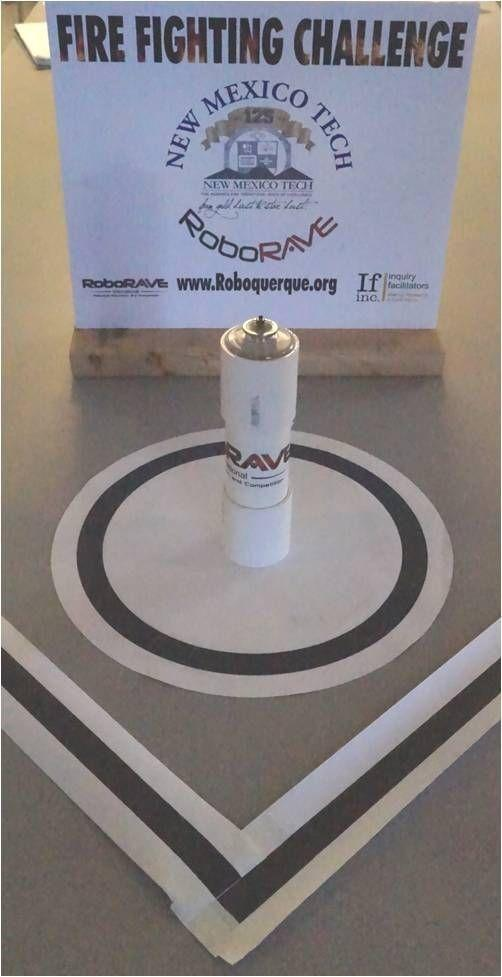
\includegraphics[width=0.4\textwidth]{images/candle.jpeg}
\end{center}
\section{Wertung}
Der "`Restzeitbonus"' wird nur dann gewährt, wenn alle vier Kerzen gelöscht sind.  Andernfalls erhält das Team nur die Punkte für gelöschte Kerzen.
\section{Strafen}
\begin{itemize}
	%\item Das System zum Löschen der Kerze wird gestartet bevor ein Teil des Roboters den weißen Kreis überquert hat. \textbf{(Kerze wird nicht gewertet)}
	%\item \textbf{Wenn eine Kerze gelöscht wurde obwohl der Roboter den weißen Kreis nicht überquert hatte erhöht sich die Punktzahl für die darauf folgende Kerze \emph{nicht}.}
	\item 50\% Abzug vom Wert der Kerze, wenn
	\begin{itemize}
		\item eine Kerze vom Roboter gelöscht wird, wenn er sich vollständig außerhalb des Kreises befindet.
		\item während des Löschvorgangs die Kerze berührt wird
	\end{itemize}
	\item Der Löschvorgang einer angezündeten Kerze ist wie folgt definiert: Eintreten in den Kreis, Löschen und Verlassen des Kreises\ldots während dieser Zeit darf der Roboter die Kerze nicht berühren.
	%\item Der Roboter berührt die Kerze während des Löschens. \emph{Der Löschvorgang gilt erst als beendet, wenn die Flamme gelöscht ist und alle Teile des Roboters außerhalb des weißen Kreises sind}. (nur 50\% der Punkte für diese Kerze)
	\item Kerzen die bereits gelöscht wurden werden zu Hindernissen und geben somit keine Strafpunkte wenn sie nach ihrem Löschvorgang berührt werden.
\end{itemize}
In der untenstehenden Bewertungsmatrix finden Sie Einzelheiten zur Bewertung der Punkte während Ihres Laufs.
\section{Punktetabelle}
\begin{center}
        \begin{tabular}{|c|c|c|c|c|c|}
	\hline \cellcolor[gray]{0.9}& \multicolumn{4}{c|}{\cellcolor[gray]{0.9}Anzahl gelöschter Kerzen} & \cellcolor[gray]{0.9} \\
	\cline{2-5} \multirow{-2}{*}{\cellcolor[gray]{0.9}} & \cellcolor[gray]{0.9}1. Kerze & \cellcolor[gray]{0.9}2. Kerze & \cellcolor[gray]{0.9}3. Kerze & \cellcolor[gray]{0.9}4. Kerze & \multirow{-2}{*}{\cellcolor[gray]{0.9}Mögliche Gesamtpunktzahl}\\
	%\cline{1-6} Außerhalb Kreis & - & - & - & - &  \multirow{3}{*}{1000}\\
        \cline{1-6} \cellcolor[gray]{0.9}\makecell{Halbe Punkte \\ aufgrund Strafabzug} & 50 & 100 & 150 & 200 &  \multirow{2}{*}{1000} \\
	\cline{1-5} \cellcolor[gray]{0.9}Volle Punktzahl & 100 & 200 & 300 & 400 & \\
        \hline \multicolumn{5}{|c|}{\cellcolor[gray]{0.9}\makecell{Zeitbonus: Die Uhr zählt von 180 Sekunden herunter und stoppt, \\ wenn der Roboter die vierte Kerze löscht.}} & 0 - 180 \\
        \hline
\end{tabular}
\end{center}
\section{Tunierplan}
\begin{itemize}
        \item Die besten acht Mannschaften werden an der Endrunde teilnehmen.
        \item Die aufsteigenden Teams werden entsprechend ihrer Gesamtpunktzahl in die Turnierliste gesetzt (siehe untenstehende Tabelle).
        \item Der zweite Platz ("`Runner Up"') wird verwendet, um den 3. Platz auf der Grundlage des Ergebnisses der Halbfinalrunde zu bestimmen.
\end{itemize}
\begin{figure}[H]
    \centering
    \def\svgwidth{\columnwidth}
    \input{tournament_score/tournament_score.pdf_tex}
\end{figure}
\end{document}
